\documentclass[a4paper, 12pt]{beamer} %%%here01

\usetheme{CambridgeUS}
\usecolortheme{beaver}
\usefonttheme{structuresmallcapsserif}


\usepackage[slovene]{babel}
\usepackage[utf8]{inputenc}
\usepackage[T1]{fontenc}
\usepackage{lmodern}
\usepackage{units}
\usepackage{eurosym}
\usepackage{amsmath}
\usepackage{amssymb}
\usepackage{amsthm}
\usepackage{amsfonts}
\usepackage{mathtools}
\usepackage{graphicx}
\usepackage{color}
%\usepackage{url}
\usepackage{enumerate}
\usepackage{enumitem}
\usepackage{pifont}

\definecolor{airforceblue}{rgb}{0.36, 0.54, 0.66}
\definecolor{bostonuniversityred}{rgb}{0.8, 0.0, 0.0}

\newcommand{\Zn}{\mathbb{Z}_n}
\renewcommand{\P}{\mathbb{P}}

\newenvironment{matematika}[1]{
\textcolor{bostonuniversityred}{\underline{\textsc{#1:}}}
}{
}

\title{Algoritem RSA}
\subtitle{Uporaba, prednosti in slabosti}
\author{Benjamin Benčina}
\institute[FMF UL]{Univerza v Ljubljani \\ Fakulteta za matematiko in fiziko \\ Oddelek za matematiko}
\date{\today}

\begin{document}
\titlepage

\begin{frame}{Uvod v kriptografijo}
\begin{itemize}[label=\ding{227}]
\item<1-> Umetnost skrivanja podatkov vsem na očeh.
\item<2-> Tajne združbe, varnostne službe, vojska, dvorci, zločinci, intelektualna elita, znanstveniki, ugankarji, računalniški protokoli...
\item<3-> Kriptanaliza - matematična sestrična tradicionalne kriptografije
\end{itemize}
\end{frame}

\begin{frame}{Kriptografija pred računalniki}
\begin{itemize}[label=\ding{227}]
\item<1-> Tajne pisave, skitala, piktogrami, premetanke...
\item<2-> Cezarjanka ($x \mapsto x + c$)
\item<3-> Vigen\`{e}rov kvadrat (urejena $n$-terica preslikav oblike $x \mapsto x + c_i$; kjer je $n$ dolžina ključa in $i \in [n]$)
\item<4-> Enigma in Alan Turing

\end{itemize}
\end{frame}

\begin{frame}{Kriptografija pred računalniki}
\framesubtitle{Turingove bombe}
\begin{minipage}[b]{0.45\linewidth}
\begin{figure}
\centering
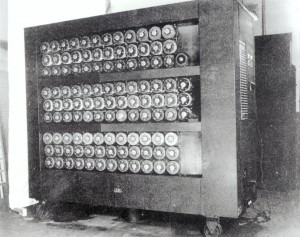
\includegraphics[scale=0.6]{turingbomb}
\caption{Ena od Turingovih bomb}
\label{fig:bomba}
\end{figure}
\end{minipage}
\hfill
\begin{minipage}[b]{0.45\linewidth}
\begin{figure}
\centering
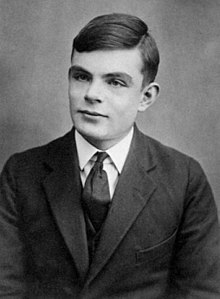
\includegraphics[scale=0.5]{AlanTuring16}
\label{fig:turing}
\caption{Alan Turing, 16 let}
\end{figure}
\end{minipage}
\end{frame}

\begin{frame}{Motivacija}
\begin{itemize}[label=\ding{227}]
\item<1->Ročne šifre so nepraktične, njihova varnost nezanesljiva.
\item<2->Mehanične šifre so drage s preveč dinamičnim algoritmom.
\item<3->Obe vrsti tradicionalnega šifriranja sta proti računalniku skoraj vedno neuporabni.
\end{itemize}
\begin{alertblock}<4->{}
\alert{Potreba po univerzalnem, matematično trdnem in varnem algoritmu.}
\end{alertblock}
\end{frame}

\begin{frame}{1978, ideja je rojena}
\begin{figure}
\centering
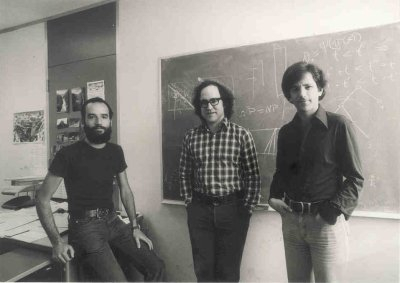
\includegraphics[scale=1.2]{rsa_inventors}
\label{fig:inventors}
\caption{Izumitelji algoritma Ronald \alert{R}ivest (sredina), Adi \alert{S}hamir (levo) in Leonard \alert{A}dleman (desno) po podelitvi patenta, 1983.}
\end{figure}
\end{frame}

\begin{frame}{Matematične osnove}
\framesubtitle{Modularna aritmetika in kolobar $\Zn$}
\begin{block}<1->{}
\begin{matematika}{definicija}
\textbf{Modularna aritmetika} (včasih tudi urna aritmetika) po modulu $n$ je aritmetika omejena s kongruenčno relacijo $a R_n b \iff n | b - a$ .
\newline
\newline
Z drugimi besedami je to aritmetika v kolobarju $\Zn$, tj. je kolobar ostankov pri deljenju celih števil z $n$, kjer je $n$ \textbf{modul}.
\end{matematika}
\end{block}

\begin{block}<2->{}
\begin{matematika}{oznake}
\newline
\begin{itemize}[label=\ding{43}]
\item Operacija $\text{mod: } \mathbb{Z} \times \mathbb{Z} \to \mathbb{Z}$ $(a, b) \mapsto \text{ostanek števila } a \text{ pri deljenju z } b$
\item Relacija $a = b \text{ (mod } n)$ pomeni, da celi števili $a$ in $b$ vrneta isti ostanek pri deljenju z $n$, oziroma mod($a$,$n$) = mod($b$,$n$).
\end{itemize}
\end{matematika}
\end{block}
\end{frame}


\begin{frame}{Matematične osnove}
\framesubtitle{Funkcija $\varphi$ in Eulerjev izrek}
\begin{block}<1->{}
\begin{matematika}{definicija}
Eulerjeva funkcija $\varphi$($n$) vrne število vseh pozitivnih celih števil manjših od $n$, ki so $n$ tuja.
\newline
\newline
$\varphi$($n$) $=$ \#\{ $a \in \mathbb{N}$; $a \leq n$, gcd($a$, $n$)$=1$\}
\end{matematika}
\end{block}

\begin{block}<2->{}
\begin{matematika}{eulerjev izrek}
Če sta si števili $x$ in $n$ tuji, velja:
\[
x^{\varphi(n)} = 1 \text{ (mod }n)
\]
\end{matematika}
\end{block}

\begin{block}<3->{}
\begin{matematika}{opomba}
$\varphi(p) = p-1$, če je $p$ praštevilo.
\end{matematika}
\end{block}
\end{frame}

\begin{frame}{Matematične osnove}
\framesubtitle{Polinomi in številski sistemi}
\begin{block}<1->{}
\begin{matematika}{definicija}
Polinom $f$ je formalna vsota $f(X) = a_0 + a_1X + \cdots + a_nX^n.$ $X$ imenujemo \emph{spremenljivka}, številom $a_i$ pravimo \emph{koeficienti}, $n$ pa je \emph{stopnja} polinoma. Vsak polinom porodi \textbf{polinomsko funkcijo}.
\end{matematika}
\end{block}

\begin{block}<2->{}
\begin{matematika}{definicija}
Število je zapisano v $n$-iškem \textbf{številskem sistemu}, $n \geq 2$, če je enako vrednosti neke polinomske funkcije iz $\Zn$ izračunane za $X = n$ in je $a_i$ števka tega števila na $i$-tem mestu, šteto od desne proti levi od $0$ naprej.
\end{matematika}
\end{block}
\end{frame}

\begin{frame}{Kako deluje?}
\begin{itemize}[label=\ding{227}]
\item<1-> Izberemo si dve različni praštevili $p$ in $q$.
\item<2-> Izračunamo $n = p \cdot q$ in $\phi(n) = \phi(p) \cdot \phi(q) = (p-1) \cdot (q-1).$
\item<3-> Izberemo naključen $e$, za katerega velja gcd($e, \phi(n)) = 1$.
\item<4-> Z razširjenim Evklidovim algoritmom poiščemo $d$, ki je multiplikativen inverz za $e$ v kolobarju $\mathbb{Z}_{\phi(n)}$. Drugače: $e \cdot d = 1 \text{ (mod } \phi(n))$.
\item<5-> Sporočilo $m$ šifriramo tako: $c = m^e \text{ mod } n$.
\item<6-> Skrito sporočilo dešifriramo tako: $m = c^d \text{ mod } n$.
\end{itemize}
\end{frame}

\begin{frame}{Zakaj deluje?}
\end{frame}

\begin{frame}{Kodiranje zaporedja znakov v števila}
\end{frame}

\begin{frame}{Načrt napada}
\end{frame}

\begin{frame}{Napad 1:}
\framesubtitle{Faktorizacija $n$, če poznamo $\phi(n)$}
\end{frame}

\begin{frame}{Napad 2:}
\framesubtitle{Kaj če sta $p$ in $q$ blizu skupaj?}
\end{frame}

\begin{frame}{Napad 3:}
\framesubtitle{Faktorizacija $n$, če poznamo $d$, oz. napad na skupen modul}
\end{frame}

\begin{frame}{Napad 4:}
\framesubtitle{Chosen-Ciphertext Attack}
\end{frame}

\begin{frame}{Napad 5:}
 \framesubtitle{Napad na majhen šifrirni eksponent $e$}
\end{frame}

\begin{frame}{Napad 6:}
\framesubtitle{Napad na majhen prostor sporočil}
\end{frame}

\begin{frame}{Napad 7:}
\framesubtitle{Napad na majhen dešifrirni eksponent $d$}
\end{frame}

\begin{frame}{Napad 8:}
\framesubtitle{Cikličen napad}
\end{frame}

\begin{frame}{Uporaba}
\end{frame}

\begin{frame}{Viri}
\end{frame}



\end{document}